\documentclass[a4paper]{article}

\setlength{\parindent}{0pt}
\setlength{\parskip}{1em}

\pagestyle{headings}

\usepackage{amssymb}
\usepackage{amsmath}
\usepackage{amsthm}
\usepackage{mathtools}
\usepackage{graphicx}
\usepackage{hyperref}
\usepackage{color}
\usepackage{microtype}
\usepackage{tikz}
\usepackage{pgfplots}
\usepackage{pgfplotstable}

\newcommand{\N}{\mathbb{N}}
\newcommand{\Q}{\mathbb{Q}}
\newcommand{\Z}{\mathbb{Z}}
\newcommand{\R}{\mathbb{R}}
\newcommand{\C}{\mathbb{C}}
\newcommand{\D}{\mathcal{D}}
\renewcommand{\S}{\mathcal{S}}
\renewcommand{\P}{\mathbb{P}}
\newcommand{\F}{\mathbb{F}}
\newcommand{\E}{\mathbb{E}}
\newcommand{\bra}{\langle}
\newcommand{\ket}{\rangle}


\graphicspath{{Image/}}

\hypersetup{
    colorlinks=true,
    linktoc=all,
    linkcolor=blue
}

\theoremstyle{definition}
\newtheorem*{axiom}{Axiom}
\newtheorem*{claim}{Claim}
\newtheorem*{conv}{Convention}
\newtheorem*{coro}{Corollary}
\newtheorem*{defi}{Definition}
\newtheorem*{eg}{Example}
\newtheorem*{lemma}{Lemma}
\newtheorem*{notation}{Notation}
\newtheorem*{prob}{Problem}
\newtheorem*{post}{Postulate}
\newtheorem*{prop}{Proposition}
\newtheorem*{rem}{Remark}
\newtheorem*{thm}{Theorem}

\DeclareMathOperator{\vdiv}{div}
\DeclareMathOperator{\grad}{grad}
\DeclareMathOperator{\curl}{curl}
\DeclareMathOperator{\Ann}{Ann}
\DeclareMathOperator{\Fit}{Fit}
\DeclareMathOperator{\Diag}{Diag}
\DeclareMathOperator{\tr}{tr}
\DeclareMathOperator{\im}{im}
\DeclareMathOperator{\Mat}{Mat}
\DeclareMathOperator{\Log}{Log}
\DeclareMathOperator{\Isom}{Isom}
\DeclareMathOperator{\Mesh}{Mesh}
\DeclareMathOperator{\Sym}{Sym}
\DeclareMathOperator{\Aut}{Aut}
\DeclareMathOperator{\cosech}{cosech}
\DeclareMathOperator{\Card}{Card}
\DeclareMathOperator{\Gal}{Gal}


\usepackage{tikzsymbols}

\setcounter{section}{-1}

\begin{document}

\title{Category Theory}

\maketitle

\newpage

\tableofcontents

\newpage

\section{Introduction}
I didn't go to the first 3 lectures, so no intro -- sorry. I have no idea on what this course is about, let's see

\newpage

\section{Definitions and examples}
\begin{defi} (1.1)\\
    A category $\mathcal{C}$ consists of:\\
    (a) a collection $\ob\mathcal{C}$ of \emph{objects} $A,B,C$;\\
    (b) a collection $\mor\mathcal{C}$ of \emph{morphisms} $f,g,h$;\\
    (c) two operations domain, codomain assigining to each $f \in \mor\mathcal{C}$ a pair of objects, its \emph{domain} and \emph{codomain}; we write $A \xrightarrow{f} B$ to mean \emph{$f$ is a morphism and $\dom f = A, \cod f = B$};\\
    (d) an operation assigning to each $A \in \ob\mathcal{C}$ a morphism $A \xrightarrow{1_A} A$;\\
    (e) a partial binary operation $(f,g) \to fg$ on morphisms, such that $fg$ is defined iff $\dom f = \cod g$, and $\dom(fg) = \dom g$, $\cod(fg) = \cod(f)$ if $fg$ is defined, satisfying:\\
    (f) $f 1_A = f = 1_B f$ for any $A \xrightarrow{f} B$;\\
    (g) $(fg) h = f(gh)$ whenever $fg$ and $gh$ are defined.
\end{defi}

\begin{rem} (1.2)\\
    (a) This definition is independent of any model of set theory. If we're given a particular model of set theory, we call $\mathcal{C}$ \emph{small} if $\ob \mathcal{C}$ and $\mor\mathcal{C}$ are sets.\\
    (b) Some texts say $fg$ means $f$ followed by $g$, i.e. $fg$ is defined iff $\cod f = \dom g$.\\
    (c) Note that a morphism $f$ is an identity iff $fg = g$ and $hf = h$ whenever the composites are defined. So we could formulate the definition entirely in terms of morphisms.
\end{rem}

\begin{eg} (1.3)\\
    (a) The category $\mathbf{Set}$ has all sets as objects, and all functions between sets as morphisms.\\
    Strictly speaking, morphisms $A \to B$ are pairs $(f,B)$ where $f$ is a set-theoretic function. (See part II logic and sets)\\
    (b) The category $\mathbf{Gp}$ has all groups as objects, group homomorphisms as morphisms.\\
    Similarly, $\mathbf{Ring}$ is the category of rings, $\mathbf{Mod_R}$ is the category of $R$-modules.\\
    (c) The category $\mathbf{Top}$ has all topological spaces as objects, and continuous functions as morphisms.\\
    Similarly, $\mathbf{Unif}$ has all uniform spaces and uniformly continuous functions as morphisms, $\mathbf{Mf}$ has all manifolds and smooth maps correspondingly.\\
    (d) The category $\mathbf{Htpy}$ has the same objects as $\mathbf{Top}$, but morphisms are homotopy classess of continuous functions. More generally, given $\mathcal{C}$, we call an equivalence relation $\simeq$ on $\mor \mathcal{C}$ a \emph{congruence} if $f \simeq g \implies \dom f = \dom g$ and $\cod f = \cod g$, and $f \simeq g \implies fh \simeq gh$ and $kf \simeq kg$ whenever the composites are defined. Then we have a category $\mathcal{C} / \simeq$ with the same objects as $\mathcal{C}$, but congruence classes as morphisms instead.\\
    (e) Given $\mathcal{C}$, the \emph{opposite category} $C^{op}$ has the same objects and morphisms as $\mathcal{C}$, but $\dom$ and $\cod$ are interchanged, and $fg$ in $\mathcal{C}^{op}$ is $gf$ in $\mathcal{C}$.\\
    This leads to the \emph{duality principle}: if $P$ is a true statement about categories, so is the statement $P^*$ obtained from $P$ by reversing all arrows.\\
    (f) A small category with one object is a \emph{monoid}, i.e. a semigroup with $1$. In particular, a group is a small cat ($\Cat$) with one object in which every morphism is an isomorphism (i.e. for all $f, \exists g$ s.t. $fg$ and $gf$ are identities).\\
    (g) A \emph{groupoid} is a category in which every morphism is an isomorphism. For example, for a topological space $X$, the \emph{fundamental groupoid} $\pi(x)$ has all points of $X$ as objects, and morphisms $x \to y$ are homotopy classes $rel\{0,1\}$ of paths $u:[0,1] \to X$ with $u(0) = x$, $u(1) = y$ (if you know how to prove that the fundamental group is a group, you can prove that $\pi(x)$ is a groupoid).\\
    (h) A \emph{discrete} cat is one whose only morphism are identities.\\
    A \emph{preorder} is a cat $\mathcal{C}$ in which, for any pair $(A,B)$, $\exists$ at most 1 morphism $A \to B$.\\
    A small preorder is a set equipped with a binary relation which is reflexive and transitive.\\
    In particular, a partially ordered set is a small preorder in which the only isomorphisms are identities.\\
    (i) The category $\mathbf{Rel}$ has the same objects as \emph{set}, but morphisms $A \to B$ are arbitrary relations $R \subseteq A \times B$. Given $R$ and $S \subseteq B\times C$, we define $S \cdot R = \{(a,c) \in A \times C | (\exists b \in B) ((a,b) \in R, (b,c) \in S)\}$.\\
    The identity $1_A:A \to A$ is $\{(a,a) | a \in A\}$.\\
    Similarly, the category $\mathbf{Part}$ are for sets and partial functions (i.e. relations s.t. $(a,b) \in R$ and $(a,b') \in R \implies b = b'$).\\
    (j) Let $K$ be a field. The cateogry $\mathbf{Mat_K}$ has natural numbers as objects, and morphism $n \to p$ are $(p \times n)$ matrices with entries from $K$. Composition is matrix multiplication.\\
    (k) We write $\mathbf{Cat}$ for the category whose objects are all small categories, and whose morphisms are functors between them. (see below for definition of functors)
\end{eg}

\begin{defi} (1.4)\\
    Let $\mathcal{C}$ and $\mathcal{D}$ be categories. A \emph{functor} $F:\mathcal{C} \to \mathcal{D}$ consists of:\\
    (a) a mapping $A \to FA$ from $\ob \mathcal{C}$ to $\ob \mathcal{D}$;\\
    (b) a mapping $f \to Ff$ from $\mor \mathcal{C}$ to $\mor \mathcal{D}$,\\
    such that $\dom(Ff) = F(\dom f)$, $\cod(Ff) = F(\cod f)$, $1_{FA} = F(1_A)$, and $(Ff)(Fg) = F(fg)$ whenever $fg$ is defined.
\end{defi}

\begin{eg} (1.5)\\
    (a) We have \emph{forgetful functors} $U$: $\mathbf{Gp} \to \mathbf{Set}$, $\mathbf{Ring}\to \mathbf{Set}$, $\mathbf{Top} \to \mathbf{Set}$, $\mathbf{Ring} \to \mathbf{AbGp}$ (forget $\times$), $\mathbf{Ring} \to \mathbf{Mon}$ (Category of all monoids) (forget $+$).\\
    (b) Given a set $A$, the free group $FA$ has the property:\\
    Given any group $G$ and any function $A \xrightarrow{f} UG$ (?), there's a unique homomorphism $FA \xrightarrow{\bar{f}} G$ extending $f$. Here $F$ is a functor $\mathbf{Set}\to \mathbf{Gp}$: given $A \xrightarrow{f} B$, we define $Ff$ to be the unique homomorphism extending $A \xrightarrow{f} B \leftrightarrow UFB$. \href{https://math.stackexchange.com/questions/1922113/what-exactly-is-functoriality}{Functoriality} follows from uniqueness given $B \xrightarrow{f} C$. $F(gf)$ and $(Fg)(Ff)$ are both homomorphisms extending $A \xrightarrow{f} B \xrightarrow{g} C \rightarrow UFC$.\\
    (c) Given a set $A$, we write $PA$ for the set of all subsets of $A$.\\
    We can make $P$ into a functor $\mathbf{Set} \to \mathbf{Set}$, given $A \xrightarrow{f} B$, we defined $Pf(A') = \{f(a) | a \in A'\}$ for $A' \subseteq A$.\\
    But we also have a functor $P^* : \mathbf{Set} \to \mathbf{Set}^{op}$ defined on objects by $P$, but $P^* f(B') = \{a \in A | f(a) \in B'\}$ for $B' \subseteq B$.\\
    By a \emph{contravariant} functor $\mathcal{C} \to \mathcal{D}$, we mean a functor $\mathcal{C} \to \mathcal{D}^{op}$ (or $\mathcal{C}^{op} \to \mathcal{D}$). A \emph{covariant} functor is one that doesn't reverse arrows (in $op$ I guess?).\\
    (d) Let $K$ be a field. We have a functor $*:\mathbf{Mod_K} \to \mathbf{Mod_K}^{op}$ defined by $V^* = \{ \text{ linear maps }  V \to K\}$, and if $V \xrightarrow{f} W$, $f^*(\theta:W \to K) = \theta f$.\\
    (e) We have a functor $op: \mathbf{Cat} \to \mathbf{Cat}$, which is the identity on morphisms (note that this is a covariant).\\
    (f) A functor between monoids is a monoid homomorphism.\\
    (g) A functor between posets is an order-preserving map.\\
    (h) Let $G$ be a group. A functor $F \circ G \to \mathbf{Set}$ consists of a set $A=F*$ together with an action of $G$ on $A$, i.e. a \emph{permutation representation} of $G$.\\
    Similarly, a functor $G \to \mathbf{Mod_K}$ is a $K$-linear representation of $G$.\\
    (i) The construction of the fundamental group $\pi(X,X)$ of a space $X$ with basepoint $X$ is a functor $\mathbf{Top}* \to \mathbf{Gp}$ where $\mathbf{Top}*$ is the category of spaces with a chosen basepoint.\\
    Similarly, the fundamental groupoid is a functor $\mathbf{Top} \to \mathbf{Gpd}$, where $\mathbf{Gpd}$ is the category of groupoids and functors between them.
\end{eg}

\begin{defi} (1.6)\\
    Let $\mathcal{C}$ and $\mathcal{D}$ be categories and $F, G: \mathcal{C}\rightrightarrows \mathcal{D}$ (why two arrows?) two functors.\\
    A \emph{natural transformation} $\alpha:F \to G$ consists of an assignment $A \to \alpha_A$ from $\ob \mathcal{C}$ to $\mor \mathcal{D}$ (think about this), such that $\dom_{\alpha_A} = FA$ and $\cod_{\alpha A} = G A$ for all $A$, and for all $A \xrightarrow{f} B$ in $\mathcal{C}$, the square 
    \begin{equation*}
        \begin{aligned}
            &FA &\xrightarrow{Ff} &FB\\
            &\downarrow \alpha_A & &\downarrow \alpha_B\\
            &GA &\xrightarrow{Gf} & GB
        \end{aligned}
    \end{equation*}
    commutes (i.e. $\alpha_B(Ff) = (Gf)_{\alpha A}$).
\end{defi}

(1.3) (l) Given categories $\mathcal{C}$ and $\mathcal{D}$, we write $[\mathcal{C},\mathcal{D}]$ for the category whose objects are functors $\mathcal{C} \to \mathcal{D}$ and whose morphisms are natural transformations.

\begin{eg} (1.7)\\
    (a) Let $K$ be a field, $V$ a vector space over $K$. There is a linear map $\alpha_V : V \to V^{**}$ given by $\alpha_V (v) \theta = \theta(v)$ for $\theta \in V^*$.\\
    This is the $V$-component of a natural transformation $1_{\mathbf{Mod_K}} \to **: \mathbf{Mod_K} \to \mathbf{Mod_K}$.\\
    (b) For any set $A$, we have a mapping $\sigma_A:A \to PA$ sending $a$ to $\{a\}$. If $f:A \to B$, then $Pf\{a\} = \{f(a)\}$. So $\sigma$ is a natural transformation $1_{\mathbf{Set}} \to P$.\\
    (c) Let $F$:$\mathbf{Set} \to \mathbf{Gp}$ be the free group functor (1.5(b)), and $U: \mathbf{Gp} \to \mathbf{Set}$ the forgetful functor. The inclusions $A \to UFA$ form a natural transformation $1_{\mathbf{Set}} \to UF$.\\
    (d) Let $G,H$ be groups and $f,g: G \rightrightarrows H$ be two homomorphisms. A natural transformation $\alpha: f \to g$ corresponds to an element $h=\alpha_*$ of $H$, s.t. $h f(x) \to g(x) h$ for all $x \in G$ or equivalently $f(x) = h^{-1} g(x) h$, i.e. $f$ and $g$ are conjugate group homomorphisms.\\
    (e) Let $A$ and $B$ be two $G$-sets, regarded as functors: $G \rightrightarrows \mathbf{Set}$. A natural transformation $A \to B$ is a function $f$ satisfying $f(g\cdot a) = g \cdot f(a)$ for all $a \in A$, i.e. a $G$-equivariant map.
\end{eg}

\begin{lemma} (1.8)\\
    Let $F,G: \mathcal{C} \rightrightarrows \mathcal{D}$ be two functors, and $\alpha: F \to G$ a natural transformation. Then $\alpha$ is an isomorphism in $[\mathcal{C},\mathcal{D}]$ iff each $\alpha_A$ is an isomorphism in $\mathcal{D}$.
    \begin{proof}
        Forward is trivial (ok, I'll check this later). For backward, suppose each $\alpha_A$ has an inverse $\beta_A$. Given $f:A \to B$ in $\mathcal{C}$, we need to show that 
        \begin{equation*}
            \begin{aligned}
                &GA &\xrightarrow{Gf} &GB\\
                &\downarrow \beta_A & &\downarrow \beta_B\\
                &FA &\xrightarrow{Ff} & FB
            \end{aligned}
        \end{equation*}
    \end{proof}
    commutes. But as $\alpha$ is natural, 
    $$(Ff)\beta_A = \beta_B \alpha_B (Ff)\beta_A = \beta_B (Gf) \alpha_A \beta_A = \beta_B (Gf)$$
    So $\beta$ is a natural transformation as well.
\end{lemma}

\begin{defi} (1.9)\\
    Let $\mathcal{C}$ and $\mathcal{D}$ be categories. By an \emph{equivalence} between $\mathcal{C}$ and $\mathcal{D}$, we mean a pair of functors $F:\mathcal{C} \to \mathcal{D}$, $G:\mathcal{D} \to \mathcal{C}$ together with natural isomorphisms $\alpha: 1_\mathcal{C} \to GF$ and $\beta: FG \to 1_\mathcal{D}$.\\
    We write $\mathcal{C} \cong \mathcal{D}$ if $\mathcal{C}$ and $\mathcal{D}$ are equivalent.\\
    We say a property $P$ of categories is a \emph{categorical property} if whenever $\mathcal{C}$ has $P$ and $\mathcal{C} \cong \mathcal{D}$, then $\mathcal{D}$ has $P$.\\
    For example, being a groupoid or a preorder are categorical properties, but being a group or a partial order are not.
\end{defi}

\begin{eg} (1.10)\\
    (a) The category $\mathbf{Part}$ is equivalent to the category $\mathbf{Set}_*$ of pointed sets (and basepoint preserving functions (as morphisms)):\\
    $\bullet$ We define $F:\mathbf{Set}_* \to \mathbf{Part}$ by $F(A,a) = A \setminus \{a\}$, and if $f:(A,a) \to (B,b)$, then $Ff(x) = f(x)$ if $f(x) \neq b$, and undefined otherwise;\\
    $\bullet$ and $G: \mathbf{Part} \to \mathbf{Set}_*$ by $G(A) = A^+ = (A \cup \{A\},A)$, and if $f:A \to B$ is a partial function, we define $Gf:A^+ \to B^+$ by $Gf(x) = f(x)$ if $x \in A$ and $f(x)$ defined, and equals $B$ otherwise.\\
    The composite $FG$ is the identity on $\mathbf{Part}$, but $GF$ is not the identity. However, there is an isomoprhism $(A,a) \to ((A \setminus \{a\})^+,A \setminus\{a\})$ sending $a$ to $A \setminus \{a\}$ and everything else to itself and this is natural.\\
    Note that there can be no isomoprhism from $\mathbf{Set}_*$ to $\mathbf{Part}$, since $\mathbf{Part}$ has a 1-element isomorphism class $\{\phi\}$ but $\mathbf{Set}_*$ doesn't.\\
    (So we see that equivalent categories can be non-isomorphic. According to a \href{https://mathoverflow.net/questions/30032/equivalence-versus-isomorphism-of-categories}{post} on SO, this usually happens when there are multiple copies of the \emph{same} thing in one but not the other. However, we can't generally \emph{discard obsolete copies} in one as that generally requires AC and is not a very useful thing to do anyway -- In short, \emph{identifying isomorphic objects is often an extremely bad idea}.)\\
    (b) The category $\mathbf{fdMod_K}$ of finite-dimensional vector spaces over $K$ is equivalent to $\mathbf{fdMod_K}^{op}$, the functors in both directions are $*$ (the dual operator) and both isomorphisms are the natural transformations of 1.7(a) (double dual).\\
    (c) $\mathbf{fdMod_K}$ is also equivalent to $\mathbf{Mat}_K$ (1.3(j)):\\
    We define $F:\mathbf{Mat_K} \to \mathbf{fdMod_K}$ by $F(n) = K^n$, and $F(A)$ is the linear map represented by $A$ w.r.t. the standard bases of $K^n$ and $K^p$.\\
    To define $G:\mathbf{fdMod_K} \to \mathbf{Mat_K}$, choose a basis for each finite dimensional vector space, and define $G(V) = \dim V$, $G(V \xrightarrow{f} W)$ to be the matrix representing $f$ w.r.t. chosen bases. $GF$ is the identity, provided we choose the standard bases for the spaces $K^n$; $FG \neq 1$, but the chosen bases give isomorphisms $FG(V) = K^{\dim V} \to V$ for each $V$, which form a natural isomorphism.
\end{eg}

---Lecture 4---

\begin{defi} (1.11)\\
    Let $\mathcal{C} \xrightarrow{F} \mathcal{D}$ be a functor.\\
    (a) We say $F$ is \emph{faithful} if, given $f,f' \in \mor \mathcal{C}$ with $\dom f = \dom f'$, $\cod f = \cod f'$, and $Ff = Ff'$, then $f=f'$ (injectivity on morphisms. The name comes more from representation theory);\\
    (b) We say $F$ is \emph{full} if, given $FA \xrightarrow{g} FB$ in $\mathcal{D}$, there exists $A \xrightarrow{f} B$ in $\mathcal{C}$ with $Ff = g$. (this is something like surjectivivity on morphisms, but see below);\\
    (c) We say  $F$ is \emph{essentially surjective} if, for every $B \in \ob \mathcal{D}$, there exists $A \in \ob \mathcal{C}$ and isomorphism $FA \to B$ in $\mathcal{D}$.\\
    We say a subcategory $\mathcal{C}' \subseteq \mathcal{C}$ is full if the inclusion $\mathcal{C}' \to \mathcal{C}$ is a full functor (basically, if the objects are kept, any morphism between them must be kept). For example, $\mathbf{Gp}$ is a full subcategory of $\mathbf{Mon}$ (the category of all monoids), but $\mathbf{Mon}$ is not a full subcategory of the category $\mathbf{SGp}$ of semigroups (consider e.g. the homomorphism that sends everything in $(\Z,\cdot)$ to $(0,\cdot)$ (which is also a semigroup); but this doesn't preserve 1 so is not a morphism in $\mathbf{Mon}$).
\end{defi}

\begin{lemma} (1.12)\\
    Assuming the axiom of choice, a functor $F:\mathcal{C} \to \mathcal{D}$ is part of an equivalence $\mathcal{C} \simeq \mathcal{D}$ if it's full, faithful, and essentially surjective.
    \begin{proof}
        $\Rightarrow$: Suppose given $G,\alpha,\beta$ as in (1.9). Then for each $B \in \ob\mathcal{D}$, $\beta_B$ is an isomorphism $FGB \to B$, so $F$ is essentially surjective.\\
        Given $A \xrightarrow{f} B$ in $\mathcal{C}$, we can recover $f$ from $Ff$ as composite $A \xrightarrow{\alpha_A} GFA \xrightarrow{GFf} GFB \xrightarrow{\alpha_b^{-1}} B$. Hence if $A \xrightarrow{f'}B$ satisfies $Ff = Ff'$, then $f=f'$. So $F$ is faithful;\\
        Lastly, for fullness, given $FA \xrightarrow{g} FB$, define $f$ to be the composite $A \xrightarrow {\alpha_A} GFA \xrightarrow{Gg} GFB \xrightarrow{\alpha_B^{-1}} B$. Then $GFf = \alpha_B f \alpha_A^{-1}$, which by construction is just $Gg$. But $G$ is faithful for the same reason as $f$, so $Ff = g$.

        $\Leftarrow$: (need to find suitable $G,\alpha,\beta$ for $F$.) For each $B \in \ob \mathcal{D}$, choose $GB \in \ob \mathcal{C}$ and an isomorphism $\beta_B : FGB \to B$ in $\mathcal{D}$. Given $B \xrightarrow{g} B'$, define $Gg:GB \to GB'$ to be the unique morphism whose image under $F$ is $FGB \xrightarrow{\beta_B} B \xrightarrow{g} B' \xrightarrow{\beta_{B'}^{-1}} FGB'$.\\
        Uniqueness implies functoriality: given $B' \xrightarrow{g'} B''$, $(Gg')(Gg)$ and $G(g'g)$ have the same image under $F$, so they are equal.\\
        By construction, $\beta$ is a natural transformation $FG \to 1_\mathcal{D}$.\\
        Given $A \in \ob \mathcal{C}$, define $\alpha_A: A \to GFA$ to be the unique morphism whose image under $F$ is $FA \xrightarrow{\beta_{FA}^{-1}} FGFA$. $\alpha_A$ is an isomorphism, since $\beta_{FA}$ also has a unique pre-image under $F$. And $\alpha$ is a natural transformation, since any naturality square for $\alpha$ (the commutative square when we defined natural transformation) is mapped by $F$ to a commutative square, and $F$ is faithful.
    \end{proof}
\end{lemma}

\begin{defi} (1.13) \\
    By a \emph{skeleton} of a category, we mean a full subcategory $\mathcal{C}_0$ containing one object from each isomorphism class. We say $\mathcal{C}$ is \emph{skeletal} if it's a skeleton of itself.\\
    For example, $\mathbf{Mat_K}$ is a skeletal, and the image of $F:\mathbf{Mat_K} \to \mathbf{fdMod_K}$ of 1.10(c) is a skeleton of $\mathbf{fdMod_K}$.\\
    (there are some examples on wikipedia)
\end{defi}

Warning: almost any assertion about skeletons is equivalent to axiom of choice (see q2 on example sheet 1).

\begin{defi} (1.14)\\
    Let $A \xrightarrow{f} B$ be a morphism in $\mathcal{C}$.\\
    (a) We say $f$ is a \emph{monomorphism} (or $f$ is \emph{monic}) if, given any pair $C \stackrel[h]{g}{\rightrightarrows} A$, $fg=fh$ implies $g=h$.\\
    (b) We say $f$ is an \emph{epimorphism} (or \emph{epic}) if it's a monomorphism in $\mathcal{C}^{op}$, i.e. if $gf = hf$ implies $g=h$.\\
    We denote monomorphisms by $A \stackrel{f}{\rightarrowtail} B$, and epimorphisms by $A \stackrel{f}{\twoheadrightarrow} B$.\\
    Any isomorphism is monic and epic: more generally, if $f$ has a left inverse (i.e. $\exists g$ s.t. $gf$ is an identity), then it's monic. We call such monomorphisms \emph{split}.\\
    We say $\mathcal{C}$ is a \emph{balanced} category if any morphism which is both monic and epic is an isomorphism.
\end{defi}

\begin{eg} (1.15)\\
    (a) As usual we consider $\mathbf{Set}$ first. In $\mathbf{Set}$, monomorphisms correspond to injections ($\Leftarrow$ is easy (ok); for $\Rightarrow$, take $C = 1 = \{*\}$), and epimorphsims correspond to surjections ($\Leftarrow$ is easy; for $\Rightarrow$, use morphisms $B \rightrightarrows 2 = \{0,1\}$). So $\mathbf{Set}$ is balanced.\\
    (b) In $\mathbf{Gp}$, monomorphisms again correspond to injections (for $\Rightarrow$ use homomorphisms $\Z \to A$); epimorphisms again correspond to surjections ($\Rightarrow$ use free products with amalgamation -- this is a non-trivial fact about groups, read more if free). So $\mathbf{Gp}$ is also balanced.\\
    (c) In $\mathbf{Rng}$ (obvious notation), monomorphisms correspond to injections (proof is much like for $\mathbf{Gp}$). However, not all epimorphisms are surjective. For example the inclusion $\Z \to \Q$ is an epimorphism, since if $\Q \stackrel[g]{f}{\rightrightarrows} R$ agree on all integers, they agree everywhere. So $\mathbf{Rng}$ is not balanced.\\
    (d) One final example is $\mathbf{Top}$. Again, monomorphisms are injections and epimorphisms are surjections (and vice versa): proof is similar to $\mathbf{Set}$ (check). However, $\mathbf{Top}$ is not balanced since a continuous bijection need not have continuous inverse.
\end{eg}

\newpage

\section{The Yoneda Lemma}
Let's not start on the content this lecture. Why are we talking about one single lemma in a chapter? Well it's not really a lemma. There's some story behind this, check here for an \href{https://www.mta.ca/~cat-dist/catlist/1999/yoneda}{obituary} which probably has the story that lecture was talking about in class.

---Lecture 5---
\begin{defi} (2.1)\\
    We say a category $\mathcal{C}$ is \emph{locally small} if, for any two objects $A,B$, the morphisms $A\to B$ in $\mathcal{C}$ form a set $\mathcal{C}(A,B)$.\\
    If we fix $A$ and let $B$ vary, the assignment $B \to \mathcal{C}(A,B)$ becomes a functor $\mathcal{C}(A,-):\mathcal{C} \to \mathbf{Set}$: given $B \xrightarrow{f} C$, $\mathcal{C}(A,f)$ is the mapping $g \to fg$. Similarly, $A \to \mathcal{C}(A,B)$ defines a functor $\mathcal{C}(-,B):C^{op} \to \mathbf{Set}$.
\end{defi}

\begin{lemma} (2.2)\\
    (i) Let $\mathcal{C}$ be a locally small category, $A \in \ob \mathcal{C}$ and $F:\mathcal{C} \to \mathbf{Set}$ a functor. Then natural transformations $\mathcal{C}(A,-) \to F$ are in bijection with elements of $FA$;\\
    (ii) Moreover, this bijection is natural in both $A$ and $F$.
    \begin{proof}
        (i) Given $\alpha$:$\mathcal{C}(A,-) \to F$, we define $\Phi(x) = \alpha_A(1_A) \in FA$. Given $x \in FA$, we define $\Psi(x): \mathcal{C}(A,-) \to F$ by $\Psi(x)_B (A \xrightarrow{f} B) = Ff(x) \in FB$.\\
        $\Psi(x)$ is natural: given $g:B \to C$, we have
        \begin{equation*}
            \begin{aligned}
                \Psi(x)_C \mathcal{C}(A,g) (f) &= \Psi(x)_C (gf) = F(gf)(x),\\
                (Fg) \Psi(x)_B(f) &= (Fg)(Ff)(x) = F(gf)(x),\\
                \Phi\Psi(x) &= \Psi(X)_A (1_A) = F(1_A)(x) = x
            \end{aligned}
        \end{equation*}
        Given $\alpha$,
        \begin{equation*}
            \begin{aligned}
                \Psi\Phi(\alpha)_B(f) \Psi(\alpha_A(1_A))_B(f) &= Ff(\alpha_A(1_A))\\
                &= \alpha_B\mathcal{C}(A,f)(1_A) = \alpha_B(f)
            \end{aligned}
        \end{equation*}
        So $\Psi\Phi(\alpha)=\alpha$.
    \end{proof}
\end{lemma}

\begin{coro} (2.3)\\
    The assignment $A \to \mathcal{C}(A,-)$ defines a full and faithful functor $\mathcal{C}^{op} \to [\mathcal{C},\mathbf{Set}]$.
    \begin{proof}
        Put $F = \mathcal{C}(B,-)$ in 2.2(i): we get a bijection between $\mathcal{C}(B,A)$ and morphisms $\mathcal{C}(A,-) \to \mathcal{C}(B,-)$ in $[\mathcal{C},\mathbf{Set}]$. We need to verify this is functorial: but it sends $f:B \to A$ to the natural transformation $g \to gf$. So functoriality follows from associativity.
    \end{proof}
\end{coro}

We call this functor (or the functor $\mathcal{C} \to [\mathcal{C}^{op}, \mathbf{Set}]$ sending $A$ to $\mathcal{C}(-,A)$) the \emph{Yoneda embedding} of $\mathcal{C}$, and denote it by $Y$.

Now let's go back to prove 2.2(ii):
\begin{proof}
    (ii) Suppose for the moment that $\mathcal{C}$ is small, so that $[\mathcal{C},\mathbf{Set}]$ is locally small. Then we have two functors $\mathcal{C} \times [\mathcal{C},\mathbf{Set}] \to \mathbf{Set}$: one sends $(A,F)$ to $FA$, and the other is the composite: $\mathcal{C} \times [\mathcal{C},\mathbf{Set}] \xrightarrow{Y \times 1} [\mathcal{C},\mathbf{Set}]^{op} \times [\mathcal{C},\mathbf{Set}] \xrightarrow{[\mathcal{C},\mathbf{Set}](-;-)} \mathbf{Set}$.\\
    2.2(ii) says that these are naturally isomorphic. We can translate this into an elementary statement, making sense even when $\mathcal{C}$ isn't small. Given $A \xrightarrow{f} B$ and $F \xrightarrow{\alpha}G$, the two ways of producing an element of $GB$ from a natural transformation $\beta:\mathcal{C}(A,-) \to F$ give the same result, namely $$\alpha_B(Ff)\beta_A(1_A) = (Gf)\alpha_A\beta_A(1_A)$$ which is equal to $\alpha_B\beta_B(f)$.
\end{proof}

\begin{defi} (2.4)\\
    We say a functor $F:\mathcal{C} \to \mathbf{Set}$ is \emph{representable} if it's isomorphic to $\mathcal{C}(A,-)$ for some $A$. By a representation of $F$, we mean a pair $(A,x)$ where $x \in FA$ is such that $\Psi(x)$ is an isomorphism.\\
    We also call $x$ a \emph{universal element} of $F$.
\end{defi}

\begin{coro} (2.5)\\
    If $(A,x)$ and $(B,y)$ are both representations of $F$, then there's a unique isomorphism $f:A \to B$ such that $(Ff)(x) = y$.
    \begin{proof}
        Consider the composite $\mathcal{C}(B,-) \xrightarrow{\Psi(y)^{-1}}F \xrightarrow{\Psi(x)} \mathcal{C}(A,-)$. By (2.3) this is of the form $Y(f)$ for a unique isomorphism $f:A \to B$, and the diagram

        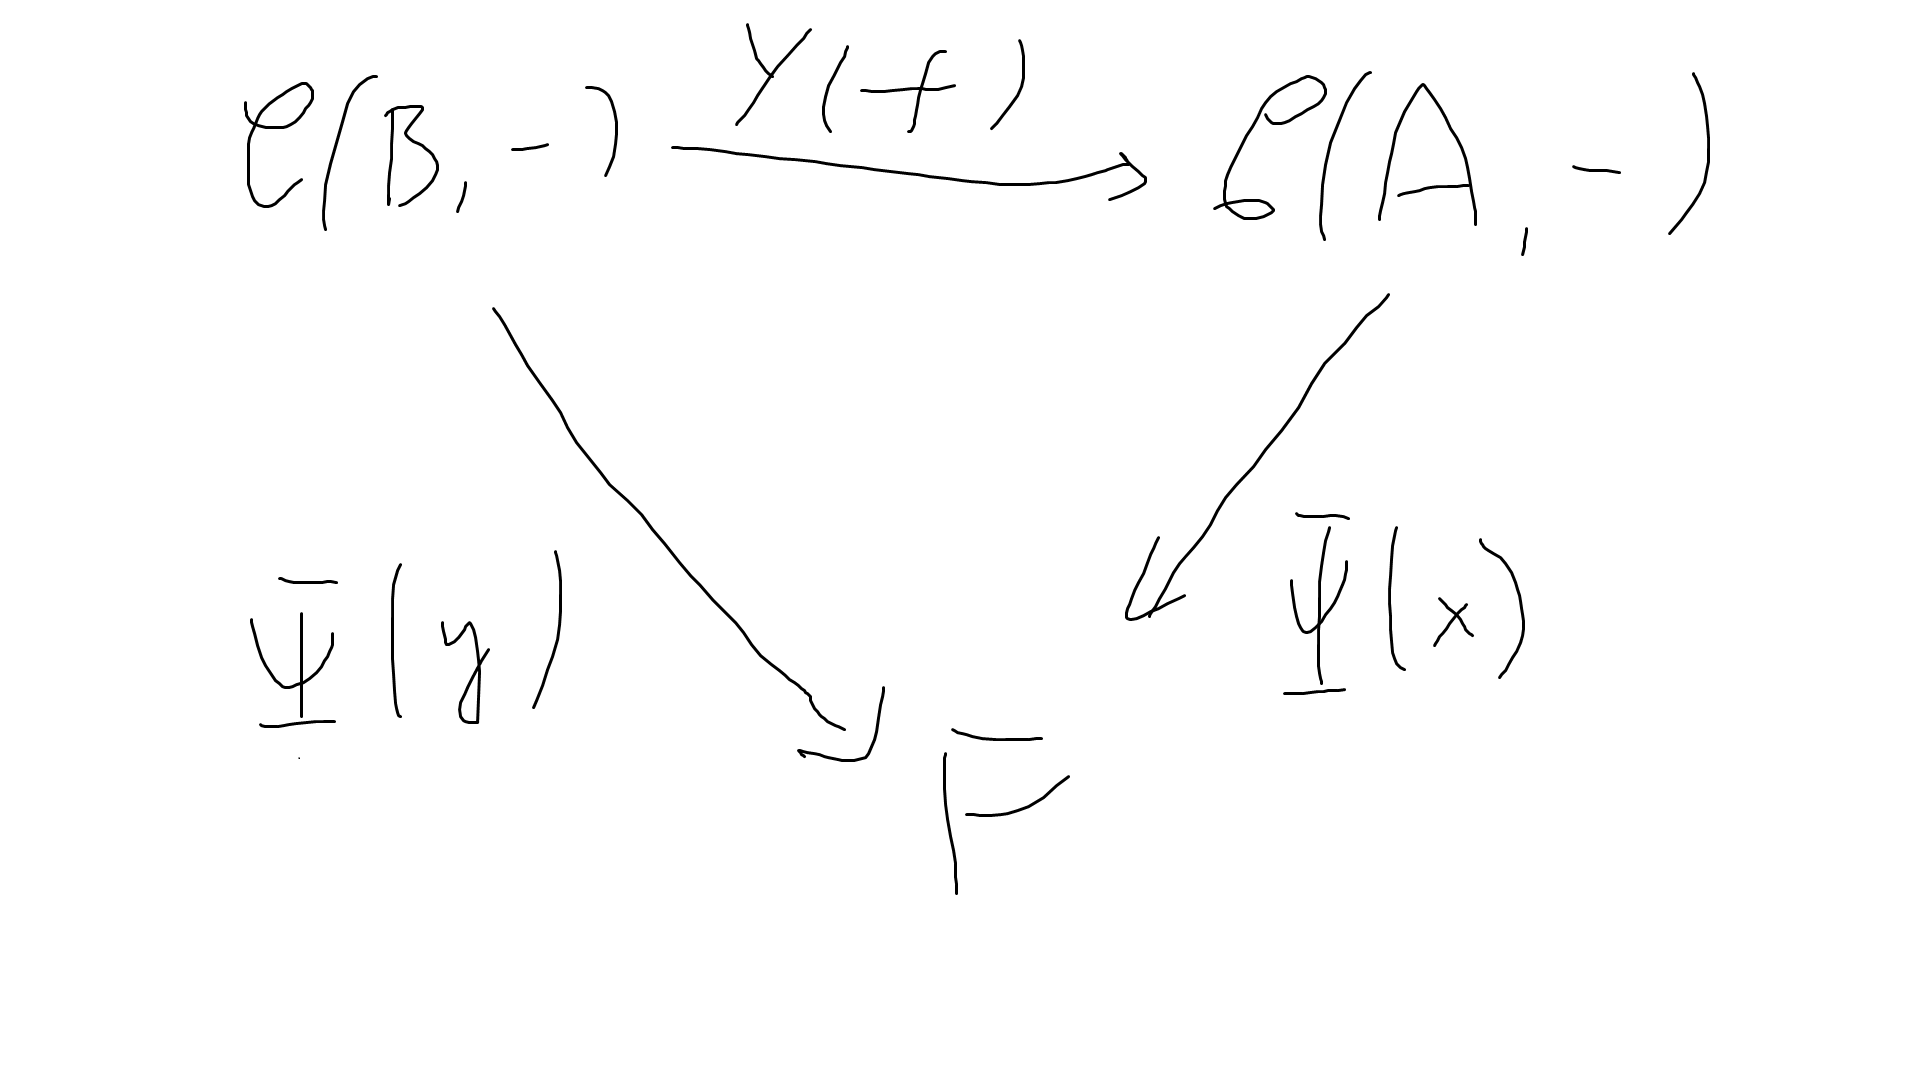
\includegraphics[scale=0.5]{image/Cat_01.png}

        commutes iff $(Ff)(x) = y$.
    \end{proof}
\end{coro}

\begin{eg} (2.6)\\
    (a) The forgetful functor $\mathbf{Gp} \to \mathbf{Set}$ is representable by $(\Z,1)$, $\mathbf{Rng} \to \mathbf{Set}$ by $(\Z[X],X])$, and $\mathbf{Top} \to \mathbf{Set}$ by $(\{*\},*)$.\\
    (b) The functor $P^*: \mathbf{Set}^{op} \to \mathbf{Set}$ is representable by $(\{0,1\},\{\mathbf{1}\})$: this is the bijection between subsets and characteristic functions.\\
    (c) Let $G$ be a group. The unique (up to isomorphism) representable functor $G(*,-): G \to \mathbf{Set}$ is the \emph{Cayley representation} of $G$, i.e. the set $\cup G$ with $G$ acting by left multiplication.\\
    (d) Let $A$ and $B$ be two objects of a small category $\mathcal{C}$. We have a functor $\mathcal{C}^{op} \to \mathbf{Set}$ sending $C$ to $\mathcal{C}(C,A) \times \mathcal{C}(C,B)$. A representation of this, if it exists, is called a (categorical) \emph{product} of $A$ and $B$, and denoted $(A \times B,(A \times B \xrightarrow{\pi_1} A, A \times B \xrightarrow{\pi_2}_B))$.\\
    This pair has the property that, for any pair $(C \xrightarrow{f}A,C\xrightarrow{g}B)$, there's a unique $C \xrightarrow{h} A \times B$ with $\pi_1 h = f$ and $\pi_2 h = g$.\\
    Products exist in many categories of interest: in $\mathbf{Set}$, $\mathbf{Gp}$, $\mathbf{Rng}$, $\mathbf{Top}$,..., they are \emph{just} cartesian products, in posets they are binary meets (see sheet 1 Q1).\\
    Dually, we have the notion of \emph{coproduct} $(A+B,A \xrightarrow{\mu_1} A + B, B \xrightarrow{\mu_2}A+B)$.\\
    These also exist in many categories of interest.\\
    ---Lecture 6---\\
    (f) (Lecturer didn't like (e) so jumped to (f) directly) Let $A \stackrel[g]{f}{\rightrightarrows} B$ be morphisms in locally small category $\mathcal{C}$. We have a functor $F:\mathcal{C}^{op} \to \mathbf{Set}$ defined by 
    \begin{equation*}
        \begin{aligned}
            F(C) = \{h \in \mathcal{C}(C,A) | fh = gh\}
        \end{aligned}
    \end{equation*}
    A representation (see (2.4)) of $F$, if it exists, is called an \emph{equalizer} of $(f,g)$: It consists of an object $E$ and a morphism $E \xrightarrow{e} A$ s.t. $fe=ge$, and every $h$ with $fh=gh$ factors uniquely (see proof of 2.9(i) which gives an insight of what this means) through $e$.\\
    In $\mathbf{Set}$, we take $E = \{x \in A | f(x) = g(x) \}$ and $e=$inclusion. Similar constructions work in $\mathbf{Gp},\mathbf{Rng},\mathbf{Top}$,...\\
    Dually, we have the notion of \emph{coequalizer}.
\end{eg}

\begin{rem} (2.7)\\
    If $e$ occurs as an equalizer, then it is a monomorphism, since any $h$ factors through it in at most one way. We say a monomorphism is \emph{regular} if it occurs as an equalizer.\\
    Split monomorphisms are regular (cf sheet1 Q6(i)).\\
    Note that regular epic monomorphisms are isomorphisms: if the equalizer $e$ of $(f,g)$ is epic, then $f=g$, so $e \cong 1_{\cod e}$.
\end{rem}

\begin{defi} (2.8)\\
    Let $\mathcal{C}$ be a category, $\mathcal{G}$ a class of objects of $\mathcal{C}$.\\
    (a) We say $\mathcal{G}$ is a \emph{separating family} for $\mathcal{C}$, if given $A \stackrel[g]{f}{\rightrightarrows} B$ such that $fh=gh$ for all $G \xrightarrow{h} A$ with $G \in \mathcal{G}$, then $f=g$.\\
    (i.e. the functors $\mathcal{C}(G,-),G \in \mathcal{G}$, are collectively faithful.)\\
    (b) We say $\mathcal{G}$ is a \emph{detecting family} if, given $A \xrightarrow{f} B$ such that every $G \xrightarrow{h} B$ with $G \in \mathcal{G}$ factors uniquely through $f$, then $f$ is an isomorphism.\\
    If $\mathcal{G} =\{G\}$, we call $G$ a \emph{separator/detector}.
\end{defi}

\begin{lemma} (2.9)\\
    (i) If $\mathcal{C}$ is a balanced category, then any saparating fmamily is detecting.\\
    (ii) If $\mathcal{C}$ has equalizers, then any detecting family is separating.
    \begin{proof}
        (i) Suppose $\mathcal{G}$ is separating and $A \xrightarrow{f} B$ satisfies the condition of 2.8(b). If $B \stackrel[h]{g}{\rightrightarrows} C$ satisfy $gf=hf$, then $gx=hx$ for every $G \xrightarrow{x} B$, so $g=h$, i.e. $f$ is epic.\\
        Similarly if $D \stackrel[l]{k}{\rightrightarrows} A$ satisfy $fk=fl$, then $ky=ly$ for any $G \xrightarrow{y} D$, since both are factorizations of $fky$ through $f$. So $k=l$, i.e. $f$ is monic.\\
        But $\mathcal{C}$ is balanced. So $f$ is an isomorphism.\\
        (ii) Suppose $\mathcal{G}$ is detecting and $A \stackrel[g]{f}{\rightrightarrows} B$ satisfies the condition of 2.8(a). Then the equalizer $E \xrightarrow{e} A$ of $(f,g)$ is isomorphism, so $f=g$.
    \end{proof}
\end{lemma}

\begin{eg} (2.10)\\
    (a) In $[\mathcal{C},\mathbf{Set}]$, the family $\{\mathcal{C}(A,-)|A \in \ob\mathcal{C}\}$ is both separating and detecting (just a restatement of Yoneda Lemma).\\
    (b) In $\mathbf{Set}$. $1=\{*\}$ (any one element set) is both a separator and a detector, since it represents the identity functor $\mathbf{Set} \to \mathbf{Set}$.\\
    Similarly, $\Z$ is both in $\mathbf{Gp}$, since it represents the forgetful functor $\mathbf{Gp} \to \mathbf{Set}$.\\
    Also, $2 = \{0,1\}$ is a coseparator and a codetector in $\mathbf{Set}$, since it represents $P^*: \mathbf{Set}^{op} \to \mathbf{Set}$.\\
    (c) In $\mathbf{Top}$, $1=\{*\}$ is a separator since it represents the forgetful functor $\mathbf{Top} \to \mathbf{Set}$, but not a detector.\\
    In fact, $\mathbf{Top}$ has no detecting \emph{set} of objects (note that this doesn't mean it has no detecting family).\\
    For any infinite cardinal $\kappa$, let $X$ be a discrete space of cardinality $\kappa$, and $Y$ the same set with \emph{co-$<\kappa$} topology, i.e. $F \subseteq Y$ is closed iff $F=Y$ or $\Card F < \kappa$ (think about, e.g. cocountable topology, then this name makes sense).\\
    The identity $X \to Y$ is continuous, but not a homeomorphism (topologically). So if $\{G_i|i \in I\}$ is any set of spaces, taking $\kappa > \Card G_i$ for all $i$ yields an example to show that the set is not detecting.\\
    (d) (some Algebraic Topology stuff) Let $\mathcal{C}$ be the category of pointed connected $CW$-complexes and homotopy classes of (basepoint-preserving) continuous mappings.\\
    JHC Whitehead proved that $X \xrightarrow{f} Y$ in this category induces isomorphisms $\pi_n(X) \to \pi_n(Y)$ for all $n$, then it's an isomorphism in $\mathcal{C}$.\\
    This says that $\{S^n | n \geq 1\}$ is a detecting set of $\mathcal{C}$.\\
    But PJ Freyd showed there is no faithful functor $\mathcal{C} \to \mathbf{Set}$, so no separating \emph{set}: if $\{ G_i | i \in I\}$ were separating, then $x \to \coprod \mathcal{C}(G_i,x)$ (disjoint unions?) would be faithful.\\
    Note that any functor of the form $\mathcal{C}(A,-)$ preserves monomorphisms, but they don't normally preserves epimorphisms.
\end{eg}

\begin{defi} (2.11)\\
    We say an object $P$ is \emph{Projective} if, given 
    \begin{equation*}
        \begin{aligned}
            &P\\
            &\downarrow f\\
            A\stackrel{e}{\twoheadrightarrow}&B
        \end{aligned}
    \end{equation*}
    (recall the two head right arrow means epimorphisms) there exists $P \xrightarrow{g} A$ with $eg = f$.\\
    (If $\mathcal{C}$ is locally small, this says $\mathcal{C}(P,-)$ preserves epimorphisms).\\
    Dually, an \emph{injective} object of $\mathcal{C}$ is a projective object of $\mathcal{C}^{op}$.\\
    Given a class $\mathcal{E}$ of epimorphisms, we say $P$ is $\mathcal{E}$-\emph{projective} if it satisfies the condition for all $e \in \mathcal{E}$.
\end{defi}

\begin{lemma} (2.12)\\
    Representable functors are (pointwise)(?) projective in $[\mathcal{C},\mathbf{Set}]$.
    \begin{proof}
        Suppose given 
        \begin{equation*}
            \begin{aligned}
                &\mathcal{C}(A,-)\\
                &\downarrow \beta\\
                F\stackrel{\alpha}{\twoheadrightarrow}&G
            \end{aligned}
        \end{equation*}
        where $\alpha$ is pointwise surjective. By Yoneda, $\beta$ corresponds to some $y \in GA$, and we can find $x \in FA$ with $\alpha_A(x) = y$. Now if $\gamma:\mathcal{C}(A,-) \to F$ corresponds to $x$, then naturality of the Yoneda bijection yields $\alpha\gamma =\beta$.
    \end{proof}
\end{lemma}

---Leture 7---
First example class: Friday 26th October, 2pm MR3.

Lecture is happy to mark any question we hand in!

\newpage

\section{Adjunctions}
\begin{defi} (3.1)\\
    Let $\mathcal{C}$ and $\mathcal{D}$ be two categories and $\mathcal{C} \xrightarrow{F} \mathcal{D}$, $\mathcal{D} \xrightarrow{G} \mathcal{C}$ two functors.\\
    By an \emph{adjunction} between $F$ and $G$ we mean a bijection between morphisms $FA \xrightarrow{\hat{f}} B$ in $\mathcal{D}$ and morphisms $A \xrightarrow{f} GB$ in $\mathcal{C}$, which is natural in $A$ and $B$, i.e. given $A' \xrightarrow{g} A$ and $B \xrightarrow{h} B'$, we have $h\hat{f} (Fg) = \widehat{(Gh)fg}: FA' \to B'$.\\
    We say $F$ is \emph{left adjoint} to $G$, and write $(F \dashv G)$.
\end{defi}

\begin{eg} (3.2)\\
    (a) The free functor $\mathbf{Set} \xrightarrow{F} \mathbf{Gp}$ is left adjoint to the forgetful functor $\mathbf{Gp} \xrightarrow{U} \mathbf{Set}$, since any functoin $f:A \to UB$ extends uniquely to a homomorphisms $\hat{f}: FA \to B$.\\
    Naturality in $B$ is \emph{easy} (lecturer says so), naturality in $A$ follows from the definition of $F$ as a functor.\\
    (b) The forgetful functor $\mathbf{Top} \xrightarrow{U} \mathbf{Set}$ has a left adjoint $D$ which equips any set with the discrete topology, \emph{and} also a right adjoint $I$ which equips a set $A$ with the discrete (lecturer had \emph{indiscrete} here?) topology $\{\phi,A\}$.\\
    (c) The functor $\ob: \mathbf{Cat} \to \mathbf{Set}$ (recall $\mathbf{Cat}$ is the category of small categories) has a left adjoint $D$ sending $A$ to the \emph{discrete} category with $\ob(DA) = A$ and only identity morphisms, and a right adjoint $I$ sending $A$ to the category with $\ob(IA) = A$ and one morphism $x \to y$ for each $(x,y) \in A \times A$. In this case $D$ in turn has a left adjoint $\pi_0$ sending a small category $\mathcal{C}$ to its set of \emph{connected components}, i.e. the quotient of $\ob\mathcal{C}$ by the smallest equivalence relation identifying $\dom f$ with $\cod f$ for all $f \in \mor \mathcal{C}$.\\
    (d) Let $M$ be the monoid $\{1,e\}$ with $e^2=e$. An object of $[M,\mathbf{Set}]$ is a pair $(A,e)$ (the images of the functor?), where $e:A \to A$ satisfies $e^2=e$.\\
    We have a functor $G:[M,\mathbf{Set}] \to \mathbf{Set}$ sending $(A,e)$ to $\{x \in A | e(x) = x \} = \{e(x) | x \in A\}$ and a functor $F: \mathbf{Set} \to [M,\mathbf{Set}]$ sending $A$ to $(A,1_A)$.\\
    I claim $(F \dashv G \dashv F)$: given $f:(A,1_A) \to (B,e)$, it must take values in $G(B,e)$, and any $g:(B,e) \to (A,1_A)$ is determined by its values on the image of $e$.\\
    (e) Let $\mathbf{1}$ be the discrete category with one object $*$. For any $\mathcal{C}$, there's a unique functor $\mathcal{C} \to \mathbf{1}$: a left adjoint for this picks out an \emph{initial} object of $\mathcal{C}$, i.e. and object $I$ s.t. there exists a unique $I \to A$ for each $A \in \ob \mathcal{C}$.\\
    Dually, a right adjoint for $\mathcal{C} \to \mathbf{1}$ corresponds to a \emph{terminal} object of $\mathcal{C}$ (think about what this means).\\
    (f) Let $A \xrightarrow{f} B$ be a morphism in $\mathbf{Set}$. We can regard $PA$ and $PB$ as posets, and we have functors $PA \stackrel[P^*f]{Pf}{\rightleftarrows} PB$.\\
    I claim $(PF \dashv P^*f)$: we have $Pf(A') \subseteq B' \iff f(x) \in B'$ for all $x \in A' \iff A' \subseteq P^* f(B')$.\\
    (g) (\emph{Galois Connection}) Suppose given sets $A,B$ and a relation $R \subseteq A \times B$. We define mappings $(-)^l$,$(-)^r$ between $PA$ and $PB$ by 
    \begin{equation*}
        \begin{aligned}
            &S^r = \{y \in B| (\forall x \in S) ((x,y) \in R) \} \text{ for } S \subseteq A\\
            &T^l = \{x \in A | (\forall y \in T) ((x,y) \in R)\} \text{ for } T \subseteq B
        \end{aligned}
    \end{equation*}
    The mappings are order-reserving (i.e. contravariant functors), and $T \subseteq S^r \iff S \times T \subseteq R \iff S \subseteq T^l$.\\
    We say $()^r$ and $()^l$ are \emph{adjoint on the right}.\\
    (h) Let's now consider, as a functor, $P^* : \mathbf{Set}^{op} \to \mathbf{Set}$ is self-adjoint on the right, since functions $A \to PB$ correspond bijectively to subsets of $A \times B$, and hence to functions $B \to PA$.
\end{eg}

\begin{thm} (3.3)\\
    (sorry I forgot to charge the other laptop today, the diagrams don't look very nice)\\
    Let $G:\mathcal{D} \to \mathcal{C}$ be a functor. Then specifying a left adjoint for $G$ is equivalent to specifying an initial object of $(A \downarrow G)$ for each $A \in \ob \mathcal{C}$, where $(A \downarrow G)$ has objects pairs $(B,f)$ with $A \xrightarrow{f} GB$, and morphisms $(B,f) \to (B',f')$ are morphisms $B \xrightarrow{g} B'$ such that 

    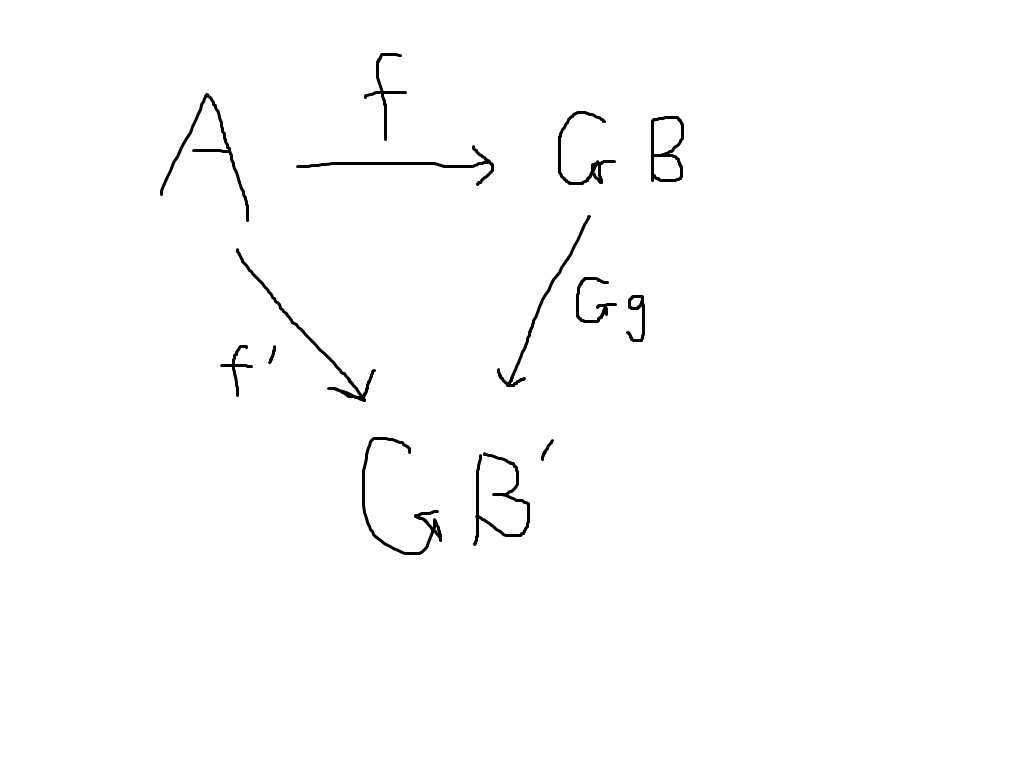
\includegraphics[scale=0.4]{image/Cat_02.png}
    
    commutes.
    \begin{proof}
        Suppose given $(F \dashv G)$. Consider the morphism $\eta_A:A \to GFA$ correspond to $FA \xrightarrow{\eta} FA$. Then $(FA,\eta_A)$ is an object of $(A \downarrow G)$. Moreover, given $g:FA \to B$ and $f:A \to GB$, the diagram 

        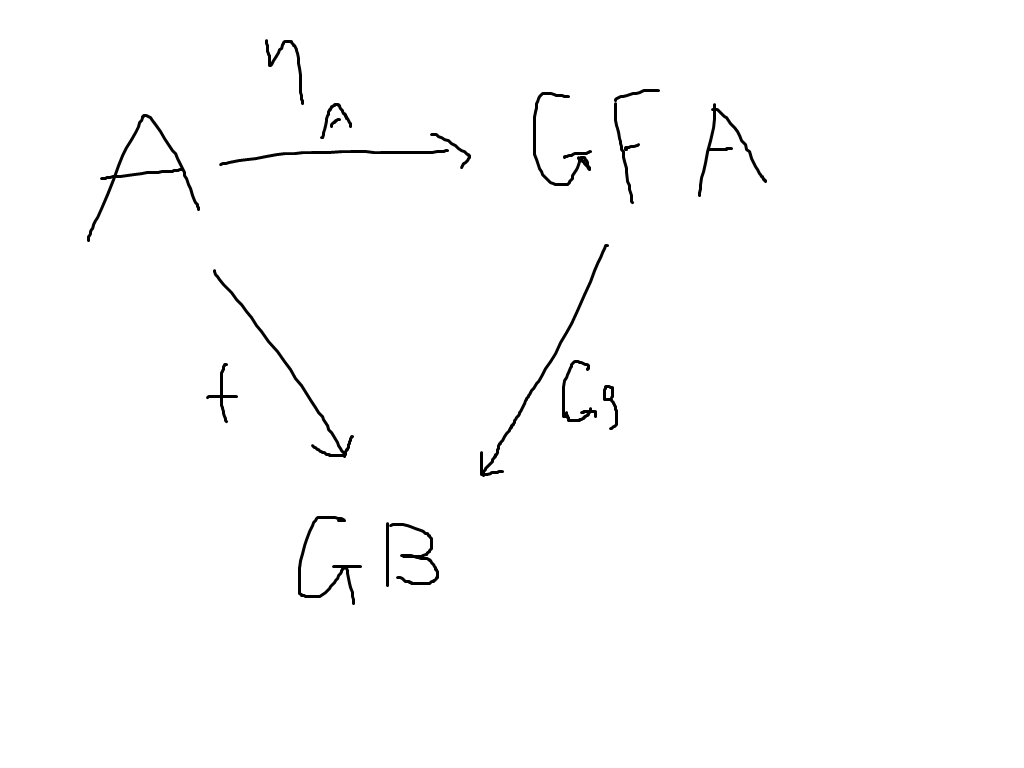
\includegraphics[scale=0.4]{image/Cat_03.png}

        commutes iff

        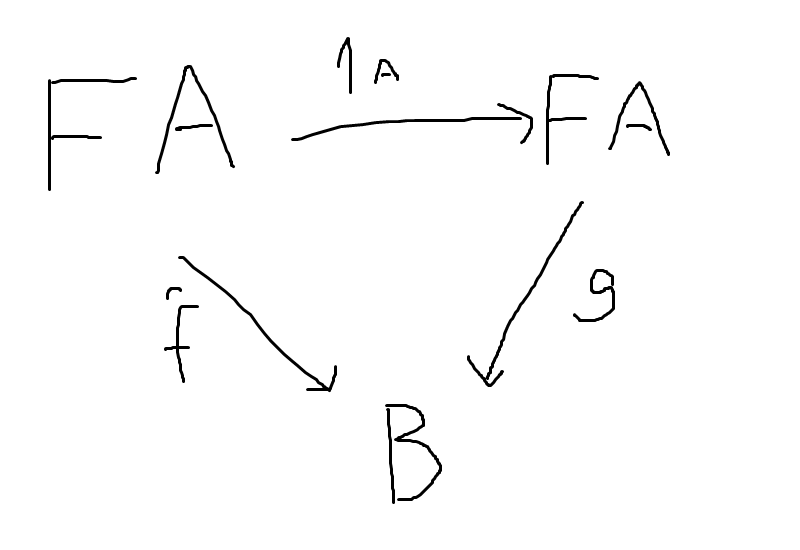
\includegraphics[scale=0.4]{image/Cat_04.png}

        commutes, i.e. $g=\hat{f}$.\\
        So $(FA,\eta_A)$ is initial in $(A \downarrow G)$.\\
        Conversely, suppose given an initial object $(FA,\eta_A)$ for each $(A \downarrow G)$. Given $A \xrightarrow{f} A'$, we define $Ff : FA \to FA'$ to be the unique morphism making 
        \begin{equation*}
            \begin{aligned}
                A & \xrightarrow{\eta_A} & GFA\\
                \downarrow f & & \downarrow GFf\\
                A' & \xrightarrow{\eta_{A'}} & GFA'
            \end{aligned}
        \end{equation*}
        commute.\\
        Functoriality follows from uniqueness: given $f': A' \to A''$, $F(f'f)$ and $(Ff')(Ff)$ are both morphisms $(FA,\eta_A) \to (FA'',\eta_{A''}F'f)$ in $(A \downarrow G)$.\\
        Note that we haven't finished: we still have to verify natural adjunctions. We'll finish off this next monday. 
    \end{proof}
\end{thm}

\end{document}
